\section{Multi-modal integration of simulated data}
Since we are unable to observe the same cell in more than one modality, simulated data is crucial for understanding and benchmarking integration methods.
Simulated data allows us to generate controlled datasets with known ground truth, allowing us to assess the performance of these integration methods and identify their strengths and limitations.
Here we mimic the properties of multi-modal single-cell datasets and compare our approach with currently available methods.

\subsection{Simulating multi-modal single-cell datasets}
 We generate three single-cell 'omics-styled technologies that share a common latent structure without direct feature correspondences using the single-cell simulation tool PROSSTT \citep{papadopoulos2019}.
Given a tree that represents some underlying branching cellular developmental process, PROSSTT parameterizes a negative binomial distribution to generate observations of cells along this trajectory.
In order to obtain three datasets that share a common latent structure yet lack any correspondences between features,  we use the same tree input but run PROSSTT under different seeds.
We utilize a five branch tree with different branch lengths (Figure \ref{fig:prosstt5-pseudotime-inverted}),
and generate high-dimensional datasets consisting of 64,000 cells with 256 markers.

\begin{figure*}[htp]
    \centering
    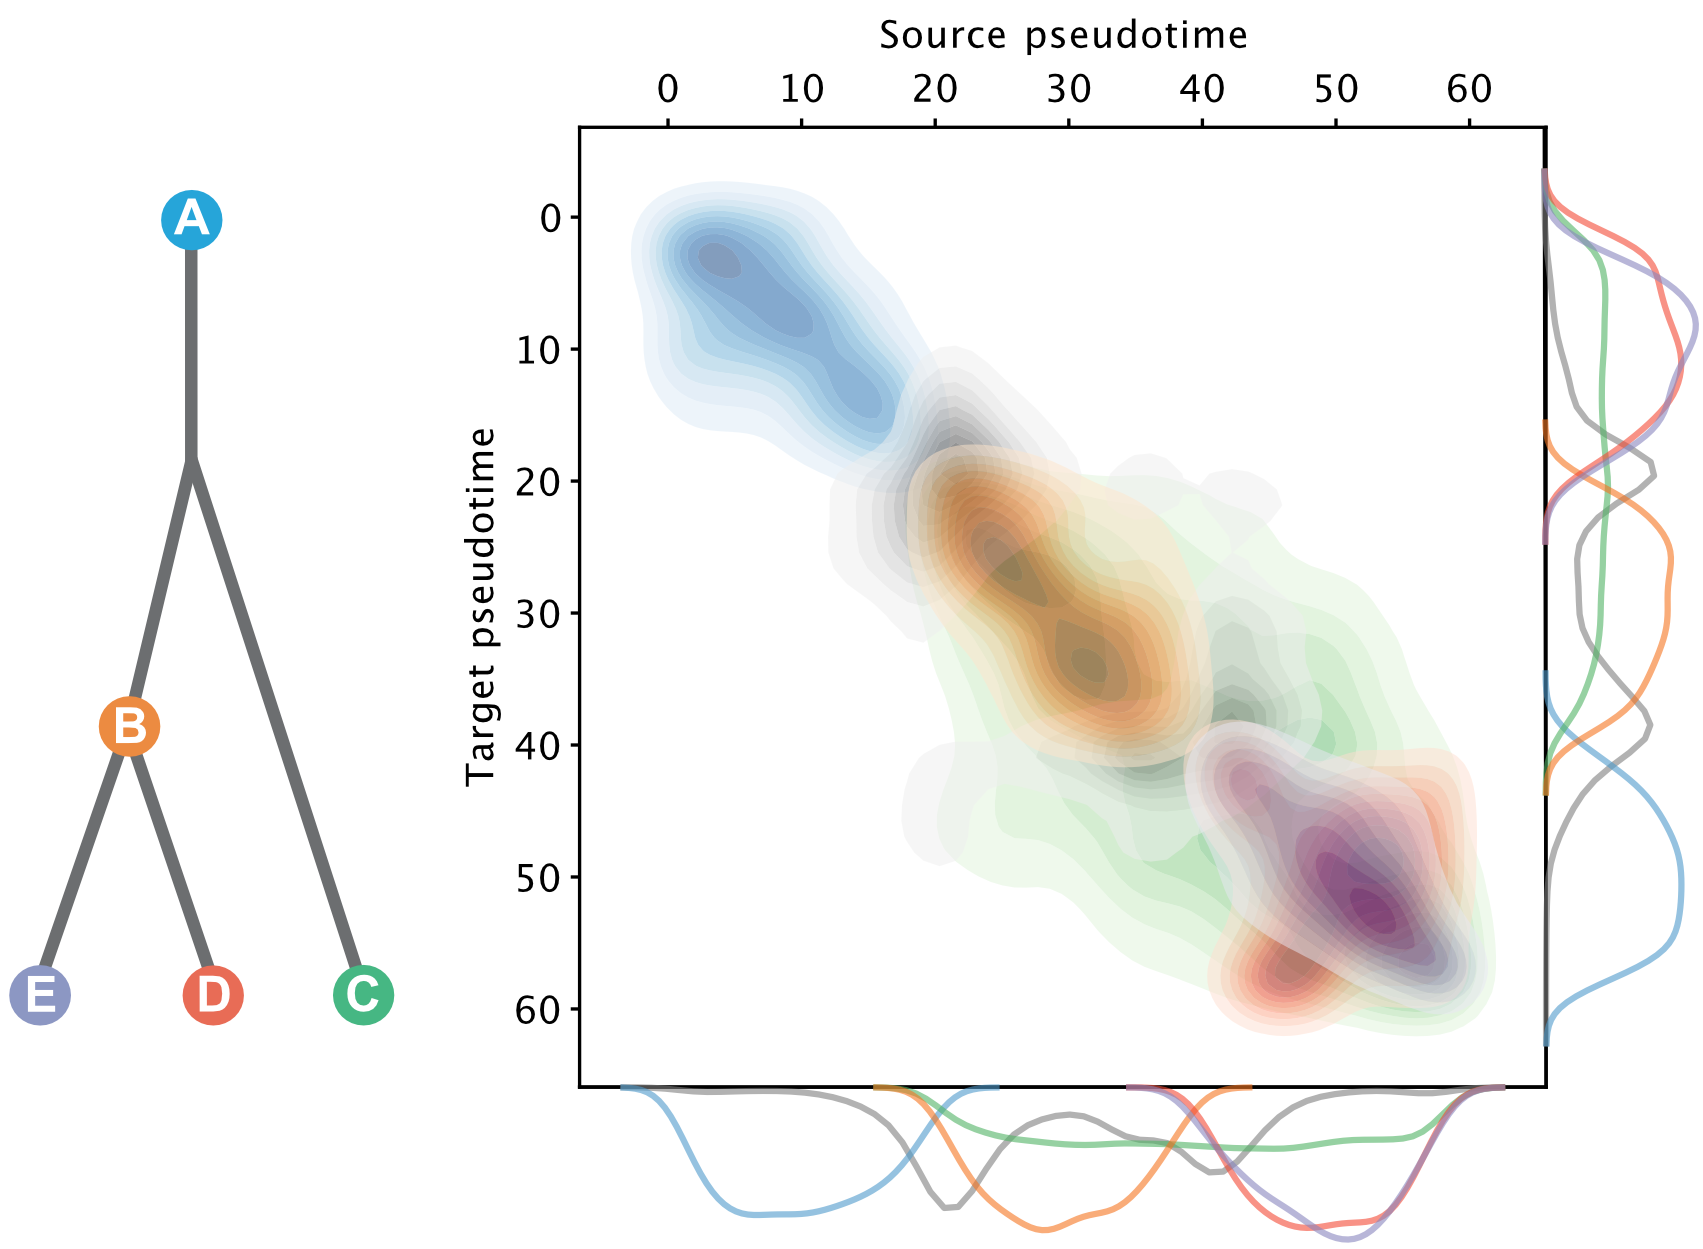
\includegraphics[width=\textwidth]{figures/integration/pseudotime-kde-tree-inverted_thick.png}
    \caption{
    Evaluation of cross-technology cell matches made by SCIM on the simulated data. The tree defining the temporal branching process underlying the simulated data is shown on the left. Cells are matched across datasets pairwise using the bipartite matching scheme and the results are depicted on the right hand-side. The Results are shown as a density plot of pseudotime values across matched cells between the source technology (x-axis) and the target technology (y-axis). Cells matched to the same branch label are colored according to the branch-color scheme (accuracy: 86\%), while mismatches are depicted in grey and appear mostly in the branching points. Marginal distributions of cell pseudotime for each branch are shown at the bottom (source technology) and left (target technology) of the density plot. We report a correlation of 0.83 (Spearman) and 0.86 (Pearson) for pseudotime label pairs.
    }
    \label{fig:prosstt5-pseudotime-inverted}
\end{figure*}


The branches in the PROSSTT tree define an overarching structure that mimics common cellular phenomena such as cell-types, while the temporal component, also called "pseudotime", provides a continuous interpolation from one branch to another, as defined by the tree  (\textbf{Figure \ref{fig:prosstt5-pseudotime-inverted}}).
In latent space, the branch structure within the data produces large clusters, while the pseudotime structure provides an \textit{orientation} within each cluster, as well as providing a global smoothing of the manifold.

\subsection{Integration with SCIM}
We apply SCIM to integrate the three simulated datasets.
The discriminator is trained to classify the source technology and is fully supervised using the branch label.
The latent space is initialized by training a VAE on the source technology.
The latent representations of the source technology are fixed,
and the two target technologies are trained for 256 epochs.
Bipartite matching is performed for each pair of datasets,
using $k=64$ and a null match penalty set to the $95^{th}$ percentile of edge costs. 

We show that SCIM embeddings capture the branching process and furthermore correctly orient the substructure of most branches (see \textbf{Figure \ref{fig:prosstt5-pseudotime-inverted}}). 
The matches retained 86\% of the branch labels correctly and give strong correlations among pseudotime values (Pearson: 0.86, Spearman: 0.83)
Furthermore, most branch mismatches occur at the nodes of the tree, where the label is ambiguous due to the continuous nature of the temporal process.

\begin{figure*}[htb]
    \centering
    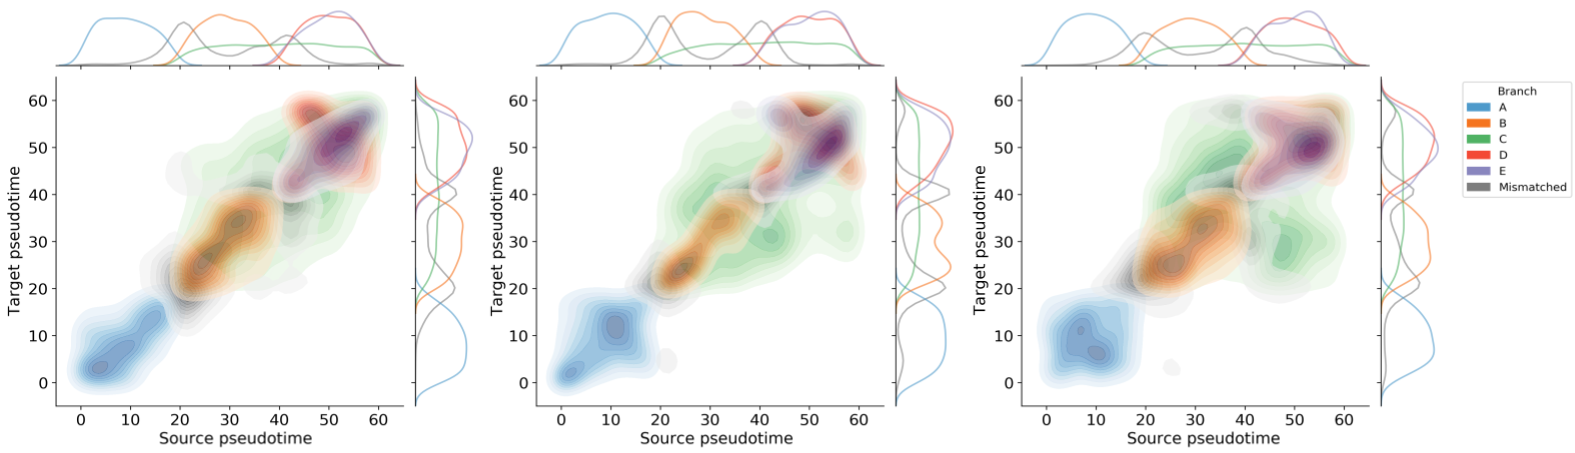
\includegraphics[width=1\textwidth]{figures/integration/3tech-pseudotime-kde.png}
    \caption{
    Evaluation of cross-technology cell matches made by SCIM on the simulated data with three technologies. 
    The pairwise matching is attained for Source-Target A, Source-Target B, and Target A-Target B, respectively. The sink edge capacities were unbounded in all cases.
    Here, we show a density plot for matched pseudotime values between the source technology and the target technology,
    colored by the branch label. Mismatched cells are colored in grey.
    The tree defining the temporal branching process can be found in Figure 3, left.
    Marginal distributions of cell pseudotime for each branch is shown on the top and right.
    }
    \label{fig:prosstt5-3tech-pseudotime}
\end{figure*}

The SCIM framework can be applied to a many-technology setting, and we demonstrate this by obtaining pairwise matches between all three datasets. 
SCIM successfully aligns the cells, based on evaluations on pseudotime (see \textbf{Supplemental Figure \ref{fig:prosstt5-3tech-pseudotime}}) as well as branch label (see \textbf{Supplemental Table \ref{tbl:prosstt_conf_SB} and  \ref{tbl:prosstt_conf_AB}}), even when using codes from such an extended latent space. 

\begin{table*}%[H]
\begin{tabular}{lrrrrr}
\toprule
Target B &     A &     B &      C &     D &     E \\
Source &       &       &        &       &       \\
\midrule
A      &  8,833 &   430 &    709 &     1 &     0 \\
B      &   249 &  6,710 &    536 &   526 &   681 \\
C      &   925 &   552 &  19,275 &     5 &     0 \\
D      &     0 &   326 &      2 &  7,906 &   314 \\
E      &     0 &   382 &      0 &   742 &  7,523 \\
\bottomrule
\end{tabular}
%\caption{Confusion table showing branch labels of the optimal matches of cells in the simulated \prost data, between Source and Target B. Entries on the diagonal correspond to correct matches whereas off-diagonal elements to mismatches. The overall accuracy, with respect to the branch label, equals 89\%.}
\label{tbl:prosstt_conf_SB}
\end{table*}

These results demonstrate that SCIM is capable of accurately identifying the best matching cells across multiple technologies, based on the shared latent representations in the presence of an underlying branching process but in the absence of paired features.

\subsection{Comparison to MATCHER}
We compare SCIM to MATCHER \citep{welch2017}, which is, to the best of our knowledge, the only other published work that can integrate multi-modal 'omics datasets in the absence of direct feature correspondences.
MATCHER, however, assumes a one-dimensional latent structure that struggles to capture hierarchical relationships, such as the ones exhibited in the simulated PROSSTT data, and frequently found and studied in single-cell datasets.
Moreover, MATCHER is built around a GPLVM \citep{lawrence2004}, which limits its scalability.
To this end, we set a budget of 48 hours compute time and limit memory consumption to 40 Gb.
Using the latent representations generated by MATCHER, we solve the bipartite matching problem setting the same hyperparameter configuration.
MATCHER is unable to model the PROSSTT branching structure and is outperformed by SCIM with respect to matching (see \textbf{Table  \ref{tbl:prosstt_matcher}} and \textbf{Figure \ref{fig:prosstt5-matcher-psuedotime}}).

%\begin{table*}%[H]
%\begin{tabular}{l|llllll}
%\toprule
%  method & accuracy & \#null matches & Spearman & Pearson \\
%\midrule
% SCIM    &   86\% &  1,590  & 0.83  & 0.86\\
% MATCHER &   4\%  & 25,510  & -0.21 & -0.19\\
%\bottomrule
%\end{tabular}
%\caption{The matching results on the PROSSTT dataset, where the SCIM matching algorithm was applied to SCIM shared latent codes and the MATCHER latent representation. The table depicts accuracy with respect to branch label, null node matches and the correlation coefficients for the pseudotime between matched source and target cells.}
%\label{tbl:prosstt_matcher}
%\end{table*}

\begin{figure*}[htp]
    \centering
    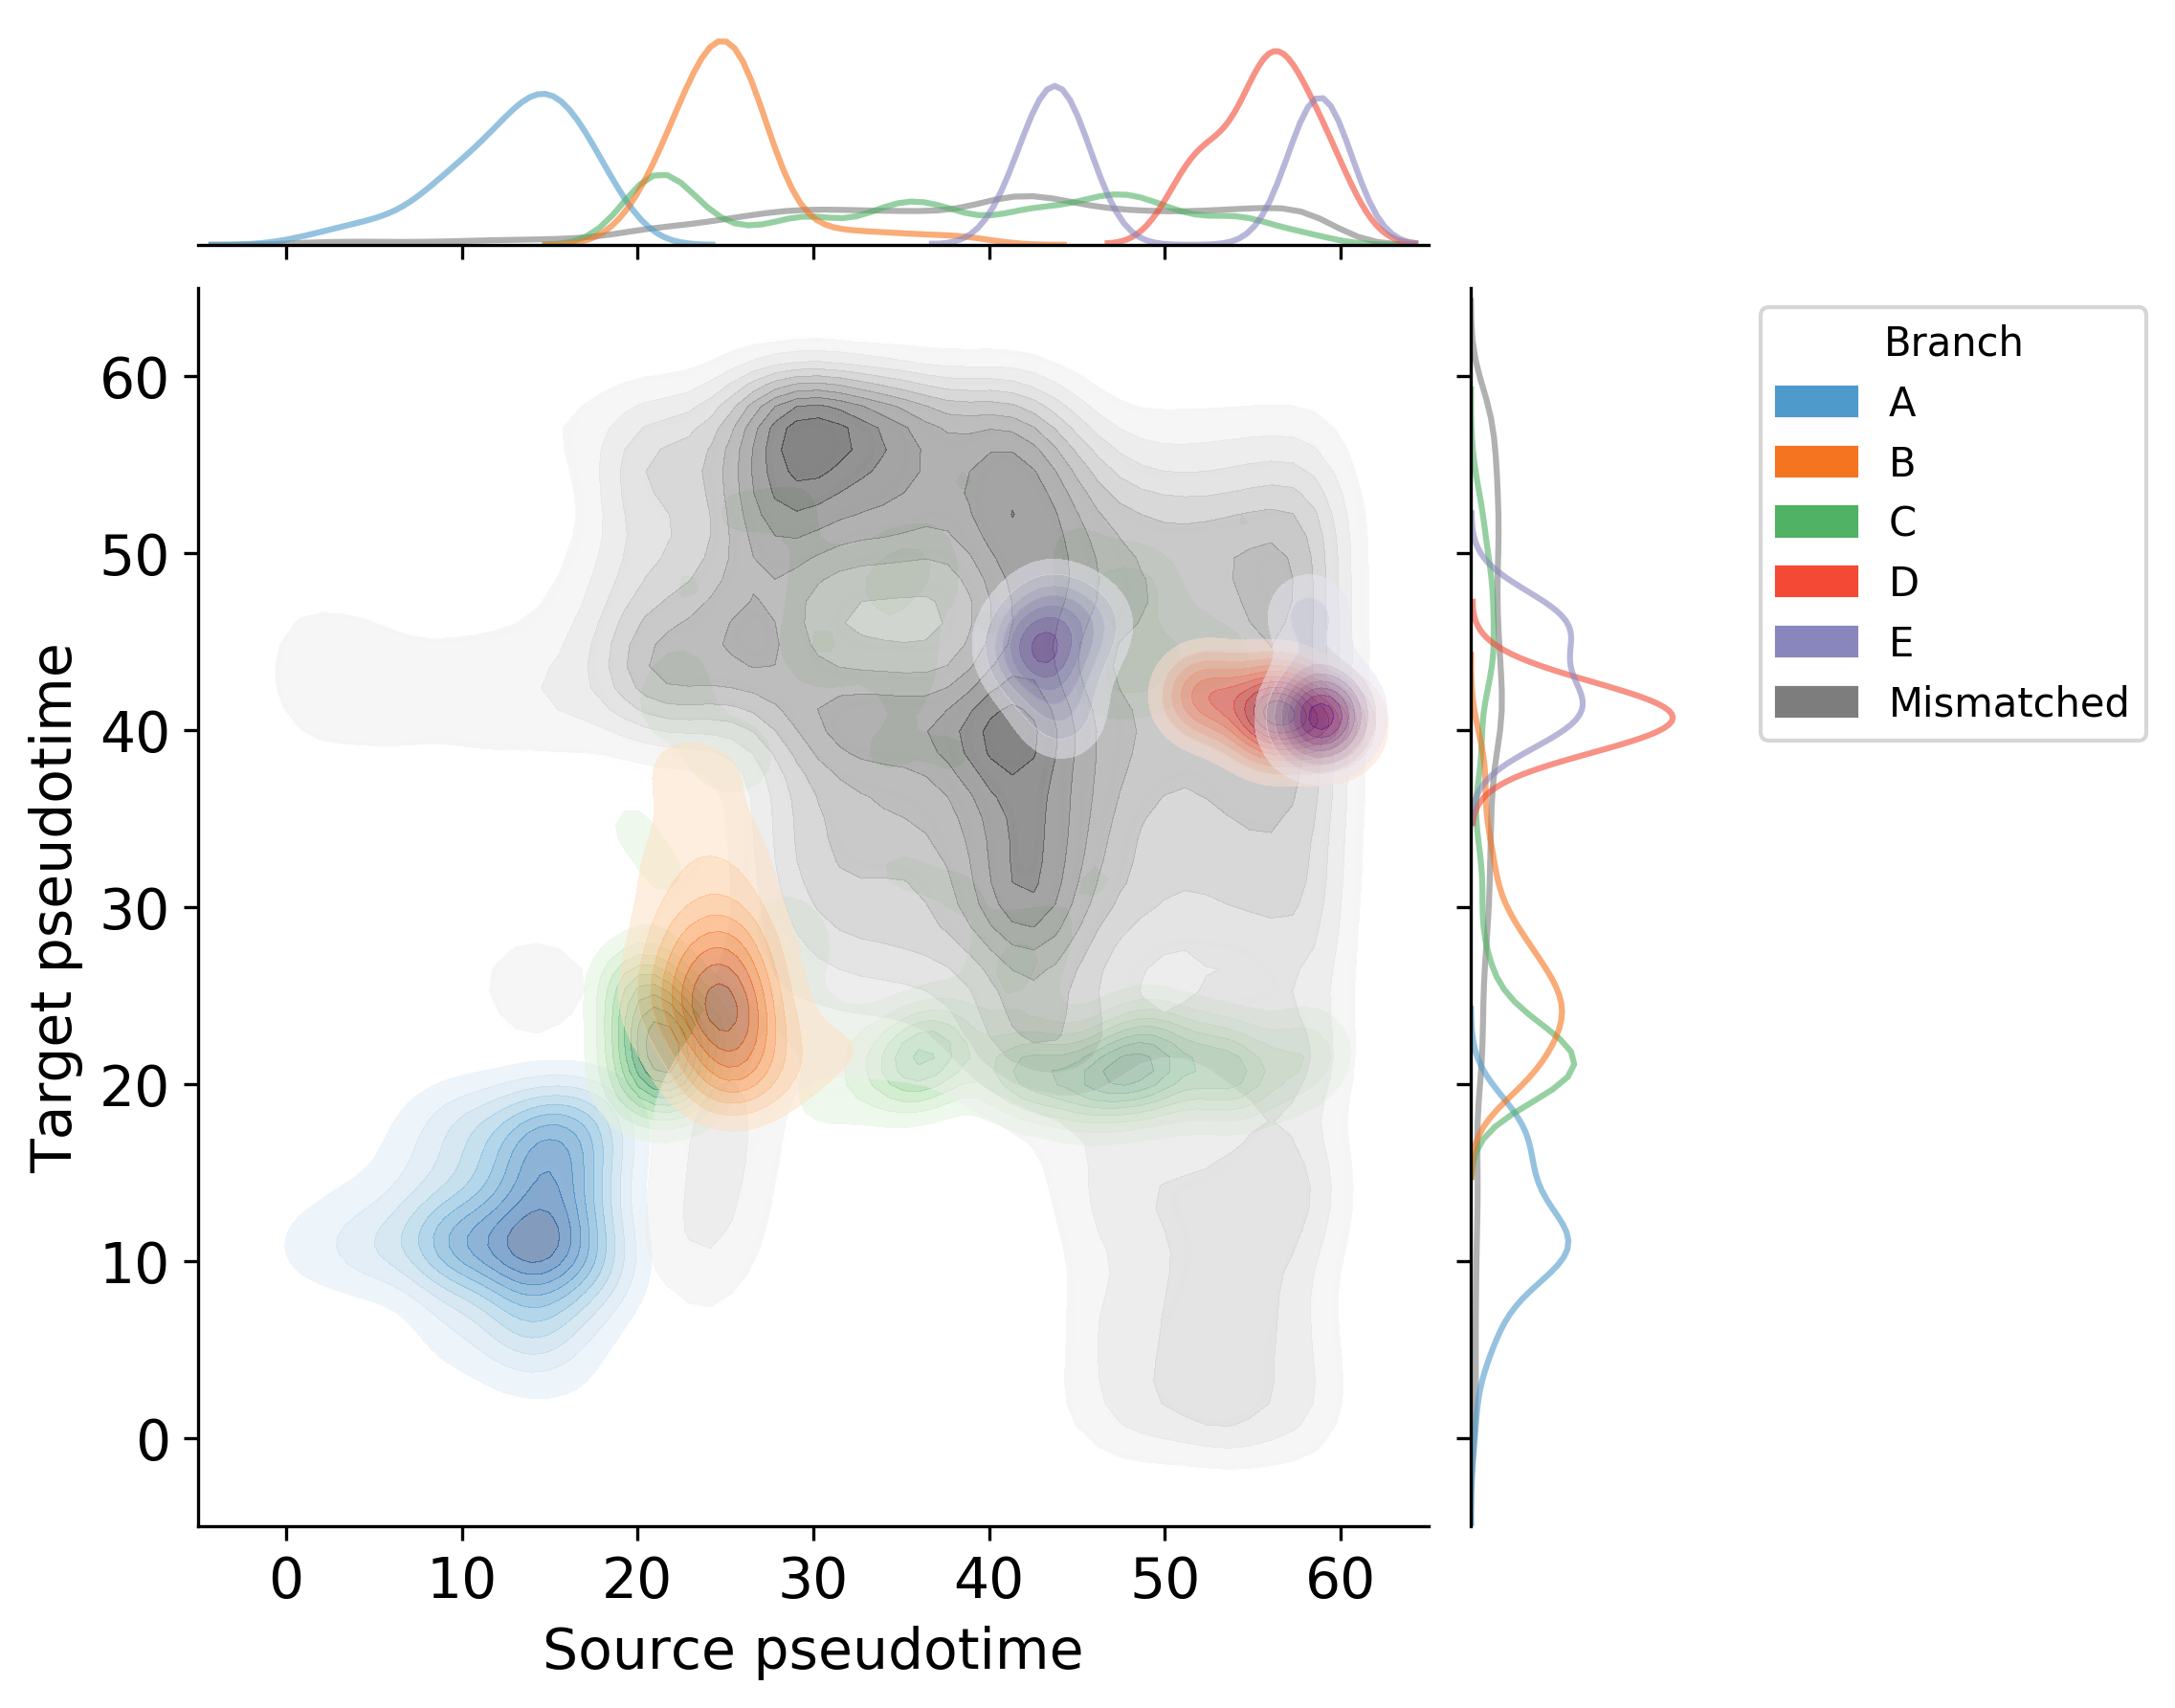
\includegraphics[width=1.0\textwidth]{figures/integration/matcher-pseudotime-kde.png}
    \caption{
    Evaluation of cross-technology cell matches using latent representation obtained by MATCHER on the simulated data.
    Cells are matched across datasets pairwise using the bipartite matching scheme.
    Here we show a density plot for matched pseudotime values between the source technology and the target technology,
    colored by the branch label. Mismatched cells are colored in grey.
    Marginal distributions of cell pseudotime for each branch are shown on the top and right.
    }
    \label{fig:prosstt5-matcher-psuedotime}
\end{figure*}
